\RequirePackage{plautopatch}

\documentclass[a4paper, 11pt]{ltjsarticle}


% マージン設定
\usepackage[top=20mm, bottom=20mm, left=20mm, right=20mm]{geometry}

% LuaLaTeX用日本語対応パッケージ
\usepackage{luatexja}
\usepackage{luatexja-fontspec}

% 必要なパッケージ
\usepackage{fontspec}
\usepackage{titlesec}
\usepackage{graphicx}
\usepackage{amsmath}
\usepackage{amssymb}
\usepackage[colorlinks=true, linkcolor=black]{hyperref}
\usepackage{tocloft}
\usepackage[english, japanese]{babel}
\usepackage{indentfirst}
\usepackage{tikz} % カスタム点線用
\usepackage{authblk} % 著者・所属パッケージ
\usepackage{here}
\usepackage{caption}
\usepackage{bookmark}

% 目次の設定
\renewcommand{\cftsecfont}{\normalsize} % セクションのフォントサイズ
\renewcommand{\cftsubsecfont}{\normalsize} % サブセクションのフォントサイズ
\renewcommand{\cftsubsubsecfont}{\normalsize} % サブサブセクションのフォントサイズ
\renewcommand{\cftsecaftersnum}{.}  % セクション番号の後にドット
\renewcommand{\cftsecpagefont}{\normalfont} % 章番号のページ番号フォントサイズ


% セクション見出しのカスタマイズ
\titleformat{\section}
  {\Large}
  {\thesection.}
  {1em}{}

\titleformat{\subsection}
  {\fontsize{11pt}{11pt}}
  {\thesubsection}
  {1em}{}

\titleformat{\subsubsection}
  {\fontsize{11pt}{11pt}}
  {\thesubsubsection}
  {1em}{}

  \setlength{\parindent}{1em}

\begin{document}

\thispagestyle{empty}
\begin{center}
\pagenumbering{gobble}  %ページ番号をカウントしない

\vspace*{40mm}
{\huge\noindent 災害時を想定したアドホックネットワーク}\\
\medskip
{\huge\noindent 構築手法の検討}\\
\vspace{\baselineskip}
{\huge\noindent\textbf{Study of Construction Methods for Ad-Hoc Network under Disaster}}\\
\vspace{120mm}

{\huge\noindent
2025年3月4日\\
東京都立産業技術高等専門学校\\
ものづくり工学科 情報通信工学コース \\
末廣 隼人\\
指導教員 髙﨑 和之    \\
}
\vspace{40mm}

\end{center}

\newpage
\thispagestyle{empty}
\tableofcontents  %目次の自動生成 目次をクリックするとその章,節に飛ぶことができる

%はじめに
\newpage
\pagenumbering{arabic}
\section{はじめに}


%理論
\newpage  %新しいページを追加
\section{理論}
\subsection{アドホックネットワークの技術的課題}
\subsubsection{隠れ端末問題}
隠れ端末問題とは、図1のようにノードAとCがノードBに対して通信を行うとき、ノードAとCはお互いの存在が隠れてしまい、
現在誰も通信を行なってないと思い込んで同時にノードBへと通信を行いデータが衝突してし壊れてしまう問題である。%
\begin{figure}[H]
  \centering
  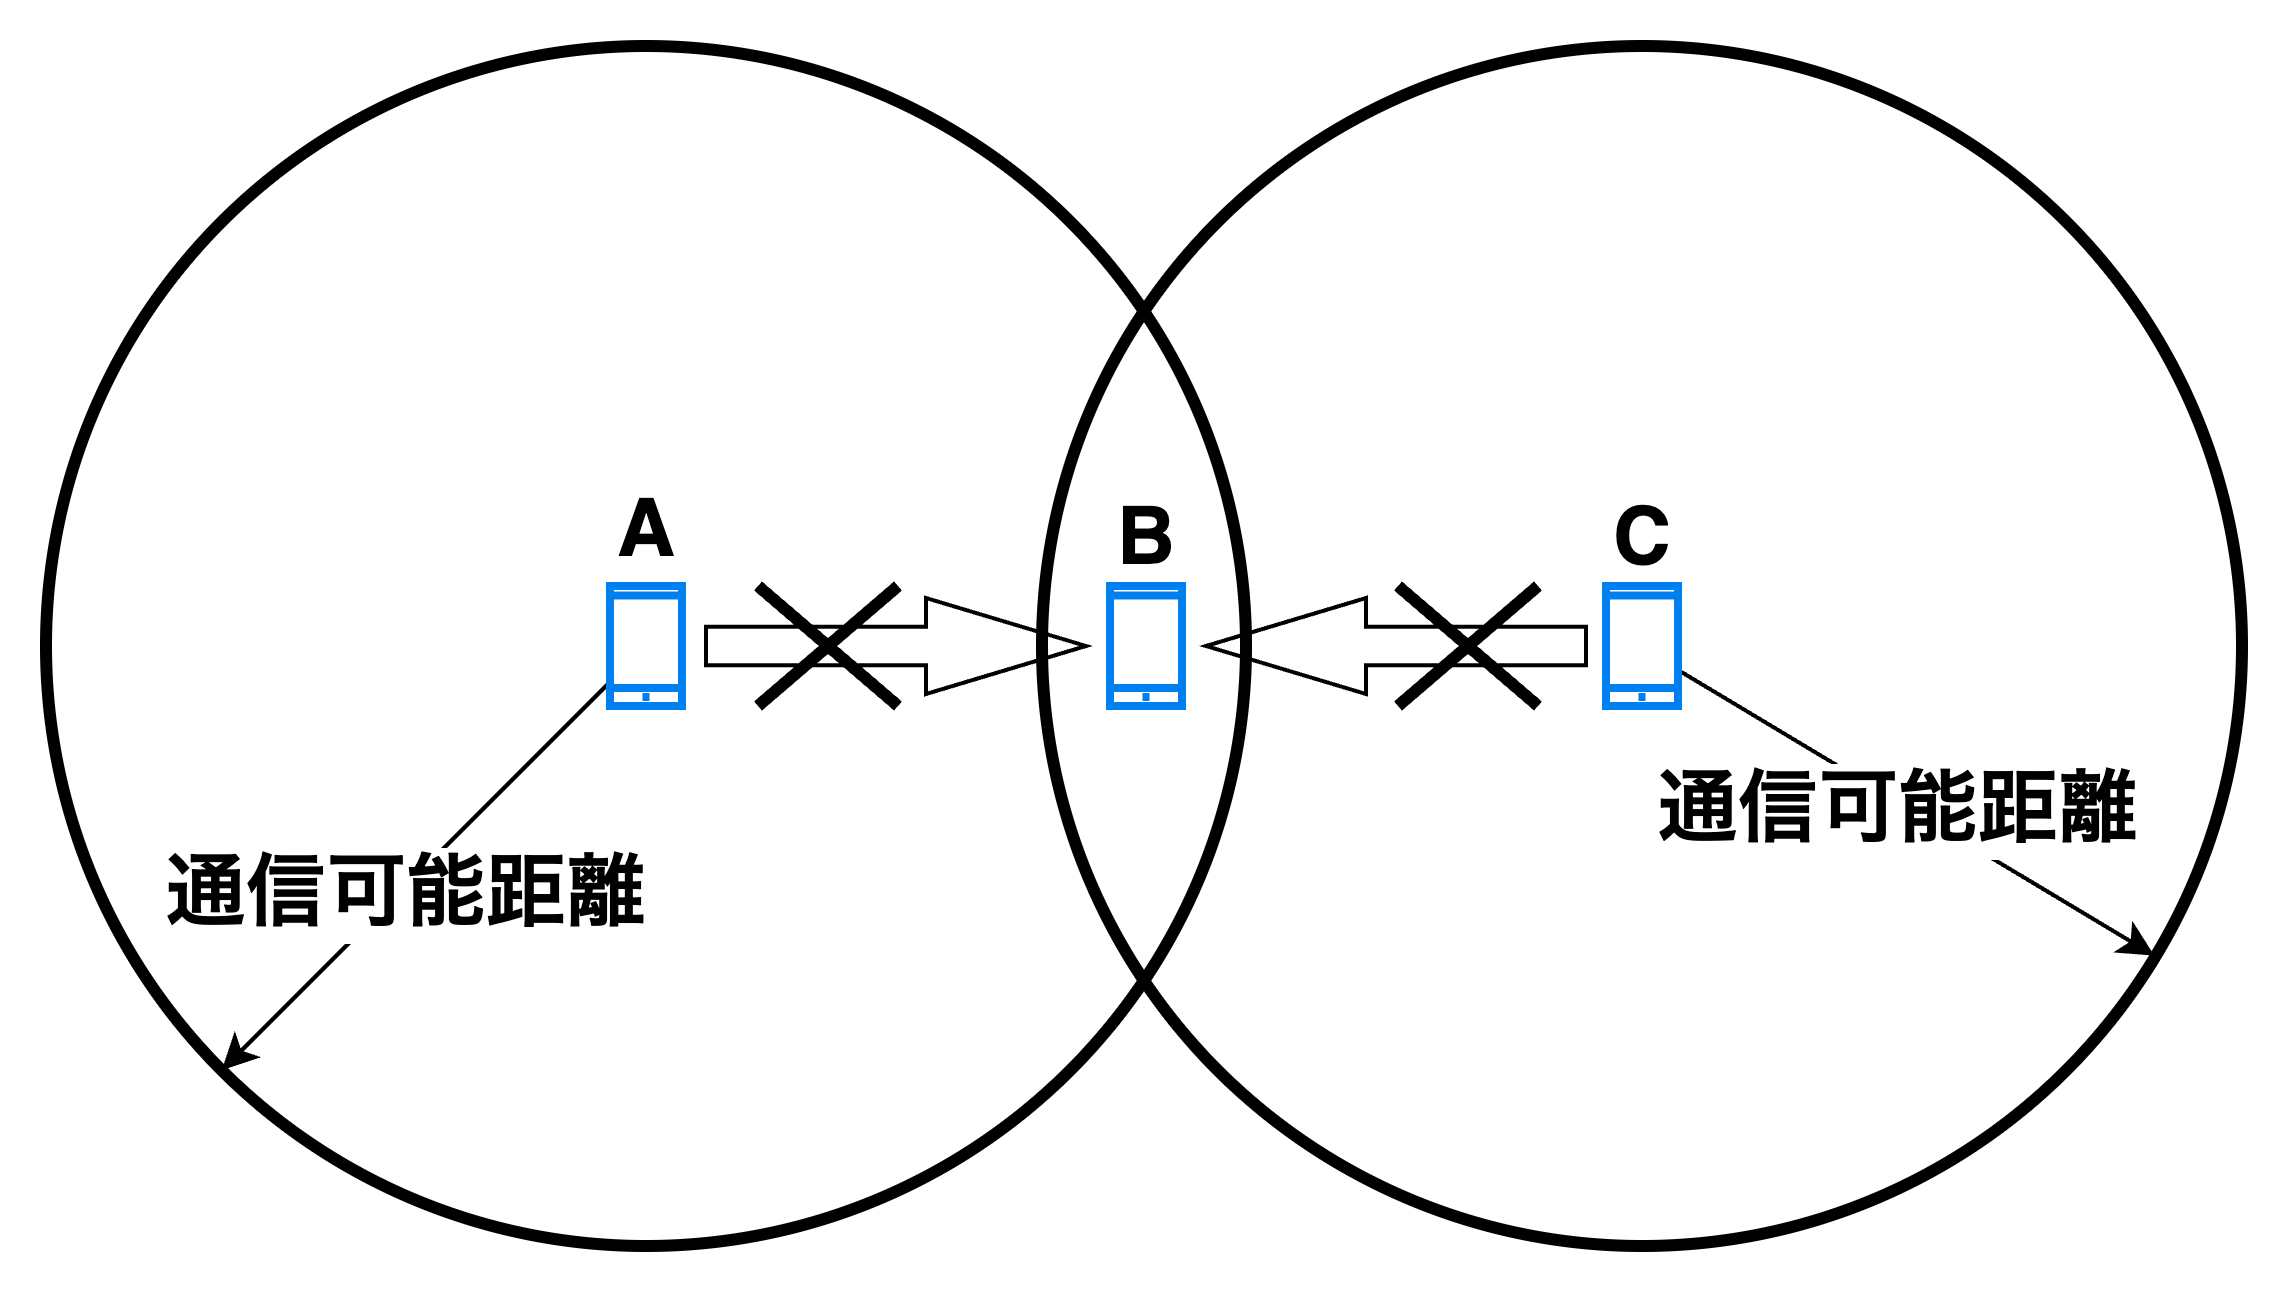
\includegraphics[width=70mm]{hidden_terminal_problem.png}
  \caption{隠れ端末問題}
\end{figure}

\subsubsection{さらし端末問題}
さらし端末問題とは、図2のようにノードAがDと通信を行なっているときノードBは端末Cと通信ができそうだが、
ノードAがDと通信を行なっているため周辺にいる他ノードは通信の抑制がされてしまい、
伝送速度や通信品質の低下が発生してしまう問題である。%
\begin{figure}[H]
  \centering
  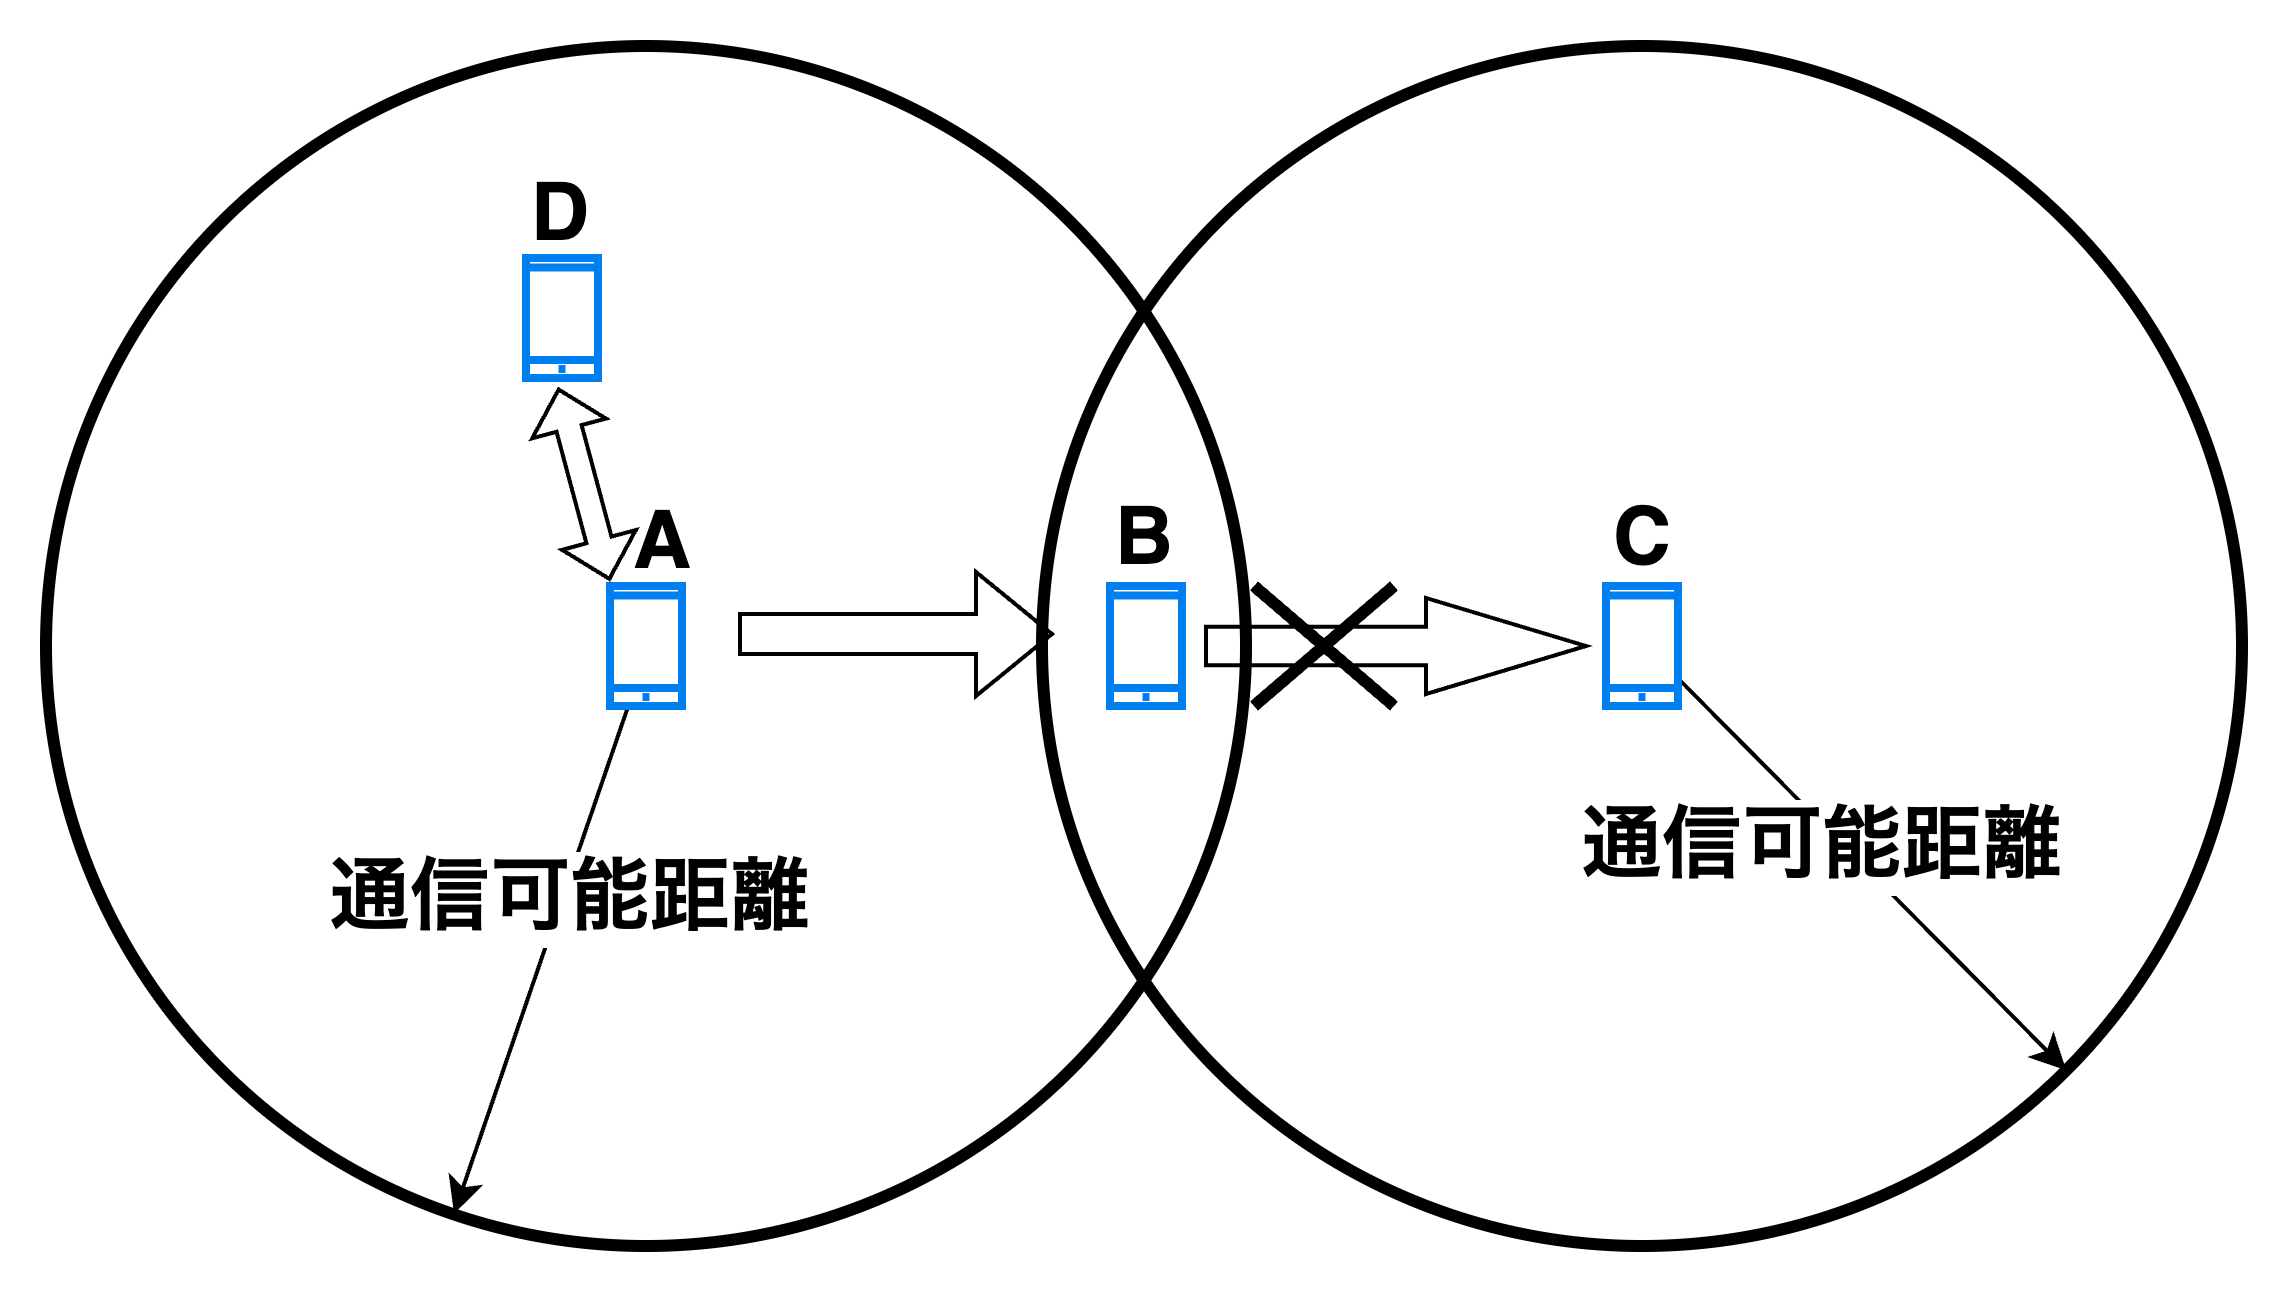
\includegraphics[width=70mm]{exposed_terminal_problem.png}
  \caption{さらし端末問題}
\end{figure}

%提案手法
\newpage
\section{提案手法}

%結果
\newpage
\section{結果}

%考察とまとめ
\newpage
\section{考察とまとめ}

%参考文献
\newpage
\section{参考文献}
\end{document}